\documentclass[tikz,border=10pt]{standalone}
\usetikzlibrary{arrows.meta, calc, positioning, quotes}

% Custom styles for nodes and arrows
\tikzset{
  block/.style={
    draw,
    rounded corners=2pt,
    minimum height=1cm,
    minimum width=1.8cm,
    font=\sffamily\footnotesize,
    align=center,
    text=black,
    fill=white,
  },
  arrow/.style={
    ->,
    >=Stealth,
    line width=1pt,
    color=black,
  },
}

\begin{document}
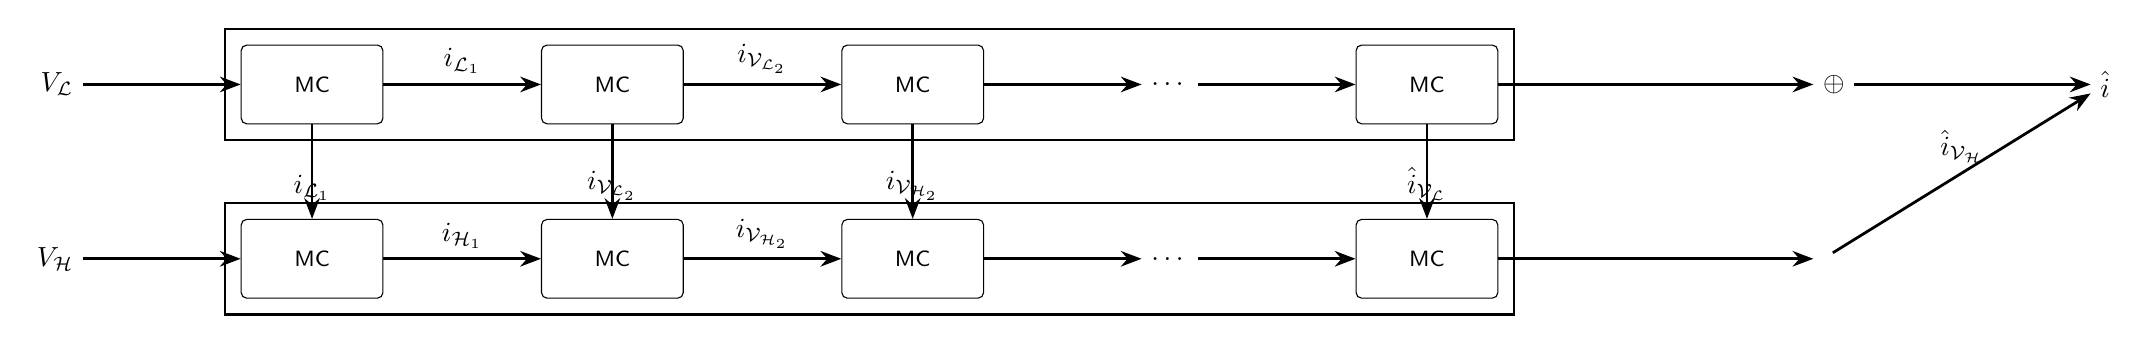
\begin{tikzpicture}[node distance=1.2cm and 2cm]

% Nodes in the top row
\node[block] (mcL1) {MC};
\node[block, right=of mcL1] (mcL2) {MC};
\node[block, right=of mcL2] (mcL3) {MC};
\node[right=of mcL3] (dots1) {\dots};
\node[block, right=of dots1] (mcLn) {MC};

% Nodes in the bottom row
\node[block, below=of mcL1] (mcH1) {MC};
\node[block, right=of mcH1] (mcH2) {MC};
\node[block, right=of mcH2] (mcH3) {MC};
\node[right=of mcH3] (dots2) {\dots};
\node[block, right=of dots2] (mcHn) {MC};

% Draw the horizontal connections in the top row
\draw[arrow] (mcL1) -- node[above] {$i_{\mathcal{L}_1}$} (mcL2);
\draw[arrow] (mcL2) -- node[above] {$i_{\mathcal{V}_{\mathcal{L}_2}}$} (mcL3);
\draw[arrow] (mcL3) -- node[above] {} (dots1);
\draw[arrow] (dots1) -- node[above] {} (mcLn);

% Draw the horizontal connections in the bottom row
\draw[arrow] (mcH1) -- node[above] {$i_{\mathcal{H}_1}$} (mcH2);
\draw[arrow] (mcH2) -- node[above] {$i_{\mathcal{V}_{\mathcal{H}_2}}$} (mcH3);
\draw[arrow] (mcH3) -- node[above] {} (dots2);
\draw[arrow] (dots2) -- node[above] {} (mcHn);

% Draw vertical connections between rows
\draw[arrow] (mcL1) -- ++(0,-1.5) -| node[pos=0.75, above] {$i_{\mathcal{L}_1}$} (mcH1);
\draw[arrow] (mcL2) -- ++(0,-1.5) -| node[pos=0.75, above] {$i_{\mathcal{V}_{\mathcal{L}_2}}$} (mcH2);
\draw[arrow] (mcL3) -- ++(0,-1.5) -| node[pos=0.75, above] {$i_{\mathcal{V}_{\mathcal{H}_2}}$} (mcH3);
\draw[arrow] (mcLn) -- ++(0,-1.5) -| node[pos=0.75, above] {$\hat{i}_{\mathcal{V}_{\mathcal{L}}}$} (mcHn);

% Input nodes V_L and V_H
\node[left=of mcL1] (VL) {$V_{\mathcal{L}}$};
\node[left=of mcH1] (VH) {$V_{\mathcal{H}}$};

% Draw input arrows
\draw[arrow] (VL) -- (mcL1);
\draw[arrow] (VH) -- (mcH1);

% Output nodes and summation symbol
\node[right=of mcLn, xshift=2cm] (sum1) {$\oplus$};
\node[right=of mcHn, xshift=2cm] (sum2) {};
\node[right=of sum1, xshift=1cm] (output) {$\hat{i}$};

% Draw output arrows
\draw[arrow] (mcLn) -- (sum1);
\draw[arrow] (mcHn) -- (sum2);
\draw[arrow] (sum1) -- (output);
\draw[arrow] (sum2) -- node[above] {$\hat{i}_{\mathcal{V}_{\mathcal{H}}}$} (output);

% Surrounding boxes
\draw[thick] ($(mcL1.north west)+(-0.2,0.2)$) rectangle ($(mcLn.south east)+(0.2,-0.2)$);
\draw[thick] ($(mcH1.north west)+(-0.2,0.2)$) rectangle ($(mcHn.south east)+(0.2,-0.2)$);

\end{tikzpicture}
\end{document}